\documentclass{thesis}

\usepackage[dvipdfmx]{graphicx}
% \usepackage[dviout]{graphicx}
% \usepackage{mediabb}
\usepackage{amsmath}
\usepackage{amssymb}
\usepackage{amsfonts}
\usepackage{amsbsy}
% \usepackage{setspace}
% \usepackage{indentfirst}
% \usepackage{subfigure}
% \usepackage{verbatim}
\usepackage{ascmac,fancybox}
% \usepackage{makeidx}
% \usepackage{enumerate}
% \usepackage{array}
\usepackage{txfonts}
\usepackage{url}
% \usepackage{multirow}
% \usepackage{float}
\usepackage{color}
% \usepackage{subfigure}
\usepackage{comment}

\def\thline{\noalign{\hrule height 1.3pt}}
\def\tvline{\vrule width 1.3pt}

% \setcounter{MaxMatrixCols}{15}
\begin{document}
% 概要
%#####################################################################
\chapter*{概要}
%#####################################################################

 インターネットの用途は幅広く,最近ではソーシャルネットワーキングサービスやクラウドサービスなどが登場したこともあり,人々がインターネットに触れる時間が長くなっている.
しかし,インターネットには少数ではあるが悪質なサイトも存在し,ウイルス感染や不正プログラムによる被害などのリスクを伴う.
情報処理通信機構から発表されている報告書では,ウイルスおよび不正プログラムの検出数は増加傾向にあり\cite{joron2},日を追うごとに脅威の危険性は高まっている.

一方で,人々はこのような脅威があるにも関わらず,脅威に関する認知および理解が十分とは言えない状況が続いている.
実際に被害やトラブルを経験したユーザの対処法で,「何もしなかった」と答えたユーザが一定数いたという報告もある\cite{joron1}.

上記の内容から,一部のユーザのコンピュータ内に,本人の意図しないうちにウイルスが潜んでいる可能性は捨てきれず,それらのコンピュータからUSBメモリやSDカードなどを通じて他のコンピュータにも感染が広がる可能性があるということは容易に想像ができる.
更にそのコンピュータが何らかのネットワークの一部であった場合,ウイルスおよび不正プログラムがネットワーク全体に打撃を与える可能性もある.
つまり,現在ネットワークを取り巻く脅威の一つとして,ネットワーク内部からの侵入も考える必要がある.
このような脅威の侵入は,一般的なファイアウォールなど外部からの侵入を監視するシステムでは防ぐことができず,ネットワーク内部にも監視・検疫を行うシステムを用意する必要がある.

本研究では,現在愛媛大学のネットワークであるEUNETを対象として新たなシステムの提案をし,そのモデルをネットワークシミュレータ上に構築した.
本論文では,シミュレータでネットワークを構築する際に作成したモジュール,および採用した考え方について述べる.

% 目次
\tableofcontents

% 序論
%#####################################################################
\chapter{���_}
%#####################################################################

% �X�肳��̓��e
\begin{comment}
�@�ߔN�C�C���^�[�l�b�g�̕��y�ɂ��C�l�b�g���[�N��𗬂��g���q�b�N���}���ɑ������Ă���D
�g���q�b�N�����̌����Ƃ��Ă�,����z�M���̃��b�`�R���e���c�̑����C�\�[�V�����l�b�g���[�L���O�T�[�r�X�ȂǑ��l�ȃA�v���P�[�V���������X�Əo����,�X�}�[�g�t�H���Ȃǂ̐V���ȃ��o�C���[���̗��p�g�傪�i��ł��邱�Ƃ���������\cite{joron1}�D

�l�b�g���[�N�����̕��G�����i�ނ��ƂŁC�l�b�g���[�N�S�̂̋��������␫�\�\��������ɂȂ��Ă��Ă���D
�l�b�g���[�N�̃g���q�b�N�������I�ɑ������Ă��邾���łȂ�,�l�b�g���[�N�̏�Ԃƃ��[�U�̐U���������ݍ�p���N����,�l�b�g���[�N���\���ł��Ȃ���ԂɊׂ邱�Ƃ��񍐂���Ă��邩��ł���\cite{joron1}�D
����ɁC���̖��̓l�b�g���[�N����K�͂ł���قnj����ƂȂ�D

�G���h�[���ԃp�X�̕����I�ȍő僌�[�g�ł��镨���ш��C�w�i�g���q�b�N�̉e�����l���������p�”\�ш悪�l�X�Ȓl�ƂȂ�C����Ɏ��ԂƂƂ��ɑ傫���ϓ����鎖���l������\cite{joron9}�D���̂悤�ɁC�l�b�g���[�N�̐U�����𗝉����鎖������ɂȂ��Ă��Ă��錻�݁C���ɑ�K�̓l�b�g���[�N�ɑ΂��鐫�\�]����@�ւ̗v�������܂��Ă���\cite{joron2}�D

�l�b�g���[�N�̐��\�]����@�Ƃ��āC���w�I��́E�V�~�����[�V�����E�����̑傫��3��ނ̎�@�����݂���D

���w�I��͂́C�ΏۂƂ���l�b�g���[�N�𐔊w�I�Ƀ��f�������邱�Ƃɂ���Ă��̐��\����͂����@�ł���C�U�镑������͓I�ɉ������Ƃ��ł���悤�ȃl�b�g���[�N�̐��\�]���ɓK���Ă���D���w�I��͂ɂ���K�̓l�b�g���[�N�̐��\�]����@�̌������ߔN�����ɍs���Ă��邪 \cite{joron3}�C���f��������ۂɑ����̋ߎ����K�v�ł��邽�ߐ��\�]�����ʂ͋ߎ��Ɉˑ����镔��������D

�V�~�����[�V�����́C�ΏۂƂ���l�b�g���[�N�̒��ۓI�ȃ��f�����v�Z�@��ɍ\�z���C�l�b�g���[�N�̋�����͋[���邱�Ƃɂ���Ă��̐��\��]�������@�ł���D���̎�@�́C���w�I��͂�����蕡�G�ȃl�b�g���[�N�̐��\�]�����”\�ł���D�����āC���ۂɋ@���p���ăl�b�g���[�N���\�z���邱�ƂȂ��C���̐��\��]�����鎖���”\�ł���D
�������C�Ώۂ����S�ɖ͋[�����V�~�����[�V�������f���𗘗p���鎖�͕s�”\�ŁC�Ώۂ̓����𒊏o�����V�~�����[�V�������f���𗘗p���Č��ʂ̌v�����s���D
�����𒊏o����ہC�ǂ̂悤�ȓ����𒊏o���邩�ɂ��V�~�����[�^��ł̌v�����ʂ��ς���Ă��܂����Ƃ���C�����ɗp�������f���̑Ó����𔻒f���鎖���K�v�ł���\cite{joron4}�D

��ʓI�Ƀl�b�g���[�N�V�~�����[�^�̓g���q�b�N���p�P�b�g�P�ʂŊǗ����邽�߁C�l�b�g���[�N�̑��x�E�K�͂��傫���Ȃ�ɂ‚�C�V�~�����[�^���Ǘ�����p�P�b�g�����������V�~�����[�V�����ɕK�v�Ȍv�Z�ʁE�������ʂ����ɑ������Ă��܂�\cite{joron5}�D���̂��ߑ�K�͂ȃl�b�g���[�N��͋[����ꍇ�C���̋K�͂ɉ������\�͂����Œv�Z�@��p�ӂ��Ȃ���΂Ȃ�Ȃ��D


�����́C���@��p���Ď��ۂɃl�b�g���[�N���\�z���邱�Ƃɂ�萫�\�]�����s�Ȃ���@�ł���D�ڍׂȐ��\�]�����”\�ł��邪�C�����ł͑����̌v�Z�@�ƃl�b�g���[�N�@���p���Ď����‹����\�z����K�v�����邽�߁C�Ǘ����w����ɑ���ȃR�X�g��v���邽�߈�ʂɂ͓���Ƃ����D�����āC�@��̌̏᎞�����Ȋ‹����ł̐��\�]�����s���ꍇ�C�Č����鎖���ɂ߂č���Ƃ�����������D���̂悤�ɁC��K�̓l�b�g���[�N�̎����͌����I�ł͂Ȃ��D�������C���Q��w�ł͕���26�N��9���ɏ��l�b�g���[�N�̍X�V���T���Ă���C�ŐV���•��G�ȃl�b�g���[�N�������‹��Ƃ��ėp���邱�Ƃ��ł���󋵂ɂ���D�{�����ł́C�V�~�����[�V�����̐��x�����߂邽�߁C�V�~�����[�V�����Ǝ��‹��Ƃ̐U�镑���̍����ŏ������鎖��ڎw���ăV�~�����[�V�����‹��̍\�z���s���D


���ۂɁC�l�b�g���[�N�V�~�����[�^�̊��p�̓l�b�g���[�N�̌�����݌v�ɂ����ė��p����鎖������D
�l�b�g���[�N�V�X�e����݌v�E�J������ہC���ۂɃl�b�g���[�N���\������O�ɃV�~�����[�V�������s���C�N���肤�錻�ۂ�����C�p�t�H�[�}���X�ɂ‚��ăV�~�����[�V�����ɂ��l�b�g���[�N���\�]���V�X�e����p���C�R���s���[�^�l�b�g���[�N�V�X�e���̐��\���l�������݌v���s�����Ƃ��d�v�ł���Ƃ����\cite{joron7}�D
�l�b�g���[�N�̌����Ɋւ��ẮC�e�햳���‹����ɂ���������擾����r�I�e�Ղł��邽�߁C�V�~�����[�^��p���ĐV�K�Z�p�̌��؂��ł��C�����p�����������s�����Ƃ��ł���\cite{joron8}�D

�{�����ł́C�V�~�����[�^��Ŏ������Q��w�l�b�g���[�N�i����EUNET�j���\�z�����\�]�����s���Ă������C����@�ցC��ƁC�������ȂǂŎg�p����Ă���l�b�g���[�N�V�~�����[�^�ɂ͔��ɐ������̂��̂�����D

���̂��߁C����̓}�C�i�[������g�p���Ȃ��C�L���E�����‹����T�|�[�g�C��K�̓l�b�g���[�N�‹����T�|�[�g�C�p�P�b�g�L���v�`���ɂ��A�j���[�V���������s�”\�C�g���[�X�o�͂��T�|�[�g�C�I�[�v���\�[�X�̖����V�~�����[�^�ł���C
�Ƃ���������S�Ė������V�~�����[�^�Ƃ���ns-3��I������D
ns-3�Ƃ́C��Ƀv���g�R�����K�̓V�X�e���‹��̌������s�������҂⋳��Ҍ����ɊJ�����ꂽ���U�C�x���g�^�l�b�g���[�N�V�~�����[�^�̂��Ƃł���D
�ڍׂɊւ��ẮC2�͂ŏq�ׂ�D�V�~�����[�V�������s���ۂ̃p�����[�^�Ƃ��ẮC�w���𗬂��g���q�b�N���v�����Đݒ肷�邱�Ƃ����z�Ƃ���邪�C
EUNET������26�N9�������\��ł��邽�߁C�{�����ł͌��݉ғ����Ă���w���l�b�g���[�N�̃g���q�b�N�ƁCEUNET�̎d�l���Ɋ�Â����@�퐫�\���p�����[�^�Ƃ��Đݒ肵�C���\�]�����s������ړI�Ƃ���D

��ʂɁC���p�^�t���[���킸�������鑽���̔ėp�l�b�g���[�N�V�~�����[�^�Ɋւ��āC���ꂼ�ꂪ�������Ă����X�̃v���g�R�����f���ɂ‚��Ă��̃��f����������ڍׁC��{�����Ƃ��������ڂ����炩�ɂ���Ă�����̂͏��Ȃ��D���̂��߁C�ėp�̕]���c�[�����g�p���ĐV���Ƀl�b�g���[�N��]������ہC���f�������@��������e�����炩�ɂȂ��Ă��邱�Ƃ��d�v���ƌ�����\cite{joron6}�D
�{�����Ɏ��������@�ɂ��Cns-3��Œ[����L2�X�C�b�`�CL3�X�C�b�`�̔ėp�I�ȃ��f�������s���C�����p���ĈӐ}�����l�X�ȃl�b�g���[�N���\�z���C���\�]�����s�����Ƃ��ł���悤�ɂȂ�D
����ɂ��Cns-3��ō\�z�����l�b�g���[�N�̋����m�F�␫�\�]���ɂ����P�_�̔������s���邾���łȂ��C�{�����Ŏg�p�����ėp�I�ȃ��f���𗘗p���C�V���ȃl�b�g���[�N�̐��\�]�����s���ۂ̃��f������C�������@�̎w�W�Ƃ��邱�Ƃ��ł���D
�����āC���N�x�ȍ~�͎��ۂɍ\�z���ꂽEUNET�̓�������؂��鎖�ŃV�~�����[�V�����ł̌v���Ǝ��@�����Ƃ��Ă̌v�����s�����Ƃ��ł��C�V�~�����[�V�������s���ہC�ǂ̂悤��EUNET�����f�������鎖�ŁC���̃��f�����Ó��������‚������؂��鎖���”\�ɂȂ�Ɨ\�z�����D

�{�_���ł́C2�͂Ɋe�V�~�����[�^�̔�r�C�V�~�����[�V�������s����ŕK�v�ƂȂ�l�b�g���[�N�Z�p�C���\�]���ʂ��Љ��D3�͂�ns-3��ł̑�K�̓l�b�g���[�N�\�z�@�ƗL���l�b�g���[�N���\�z���邽�߂ɍ쐬�������W���[���C4�͂ɍ쐬�������W���[���̓��쌟�؂ɂ‚��ďq�ׁC�Ō��5�͂ł܂Ƃ߂ƍ���̉ۑ���q�ׂ�D
\end{comment}

% �����̓��e
�ߔN�C

% 関連研究
%#####################################################################
\chapter{関連技術}
%#####################################################################

 本研究では,提案したネットワークモデルをネットワークシミュレータを用いて構築しシミュレーションを行う.
本章では,2.1節で使用するネットワークシミュレータの説明を行い,2.2節ではOpenFlow技術の説明をし,最後に2.3節では,ネットワークモデルを構築する際に必要となるネットワークの諸技術を説明する.

\section{ネットワークシミュレータ ns-3}

ns-3(Network Simulator Version 3)\cite{ns3} \cite{ns3text} とは,その前身であるns-2の開発に携わっている主要メンバーにより開発された,オープンソースベースの離散イベント駆動型シミュレータである.
ns-3の開発チームには,Tom Henderson主任研究員を筆頭に,副主任研究員としてSumit Roy(ワシントン大学),George Riley(ジョージア工科大学),Sally Floyd(カリフォルニア大学バークレイ分校ISCIセンター)など,ネットワークの研究分野において著名な研究者たちが名を連ねている.
無料で使用可能なシミュレータながら,最新のサービスやプロトコルのサポートを行うなどの積極的な開発を行っているため,近年では一般的になりつつある.

ns-3では,有線でのパケット通信しか想定されていなかったなど数々あったns-2の問題点を解消し,ns-2の開発時点では存在しなかった新たなプロトコルの実装および,より大規模なシミュレーションの評価をより簡単にする目的で開発された.
このとき,ns-2でのシナリオ記述で採用していたObject TCL言語の使用を廃止し,事実上C++言語を用いたデザインに統一したため,ns-3とns-2の間の互換性が無くなってしまった.
そのため,有線ネットワーク系のシミュレーションにはns-2を,無線ネットワーク系および比較的新しい技術を用いたネットワークのシミュレーションにはns-3を使うのが一般的であったが,現在では,ns-2の機能の完全移植が着実に進んでおり,徐々にns-3のシェアが高まっている. \\

ns-3には,本研究で用いるOpenFlowに対応しているほかに,以下の機能を備える.

\subsubsection{Pythonによるシナリオファイルの作成}

ns-3は,C++言語でのデザインに統一されたが,シミュレーションするネットワークモデルの構築を行うシナリオファイルの記述には,簡易スクリプト言語であるPythonも使用することができる.
Pythonを用いてシナリオファイルを作成することによって,コード量の削減および可読性が高まり,第三者が見ても分かりやすいシナリオファイルを作成することができる.

本研究では,ns-3がOpenFlowのPythonバインディングに対応していないということと,Pythonの欠点である実行速度の遅さが如実に表れる可能性があるということから,C++言語を用いてシナリオファイルのコーディングを行っている.

\subsubsection{tcpdumpを用いたトレースファイルの解析}

シナリオファイルにトレースファイルの生成を可能にするコードを追加することで,シナリオに存在する全てのノードの全てのデバイスに対して,パケットの入力,出力のデータを持つパケットキャプチャ用ライブラリのlibpcap形式(以下,PCAP形式)のトレースファイルを生成することができる.
これをLinuxに標準搭載されているキャプチャツールであるtcpdumpを用いることで,PCAP形式のトレースファイルを解析することが可能である.

\subsubsection{シミュレーション結果の可視化}

ns-3では,PyVizというライブラリを用いることによって,トレースファイルを用いたシミュレーション結果のアニメーション表示が可能である.
PyVizは最新のns-3パッケージに標準搭載されており,パケットの通信経路,パケットの転送速度などを可視化して表示することができ,シミュレーション結果の時間的な流れを柔軟に変更させながら,結果の解析ができる.

\subsubsection{実機を用いたシミュレーション}

ns-3には,LinuxなどのUNIX系OSに搭載されているTAPデバイスを用いて,現実で動作しているホストやデバイスなどをシミュレーション内に統合させることができる.
これを用いることによって,実際に稼働しているパケット通信をシミュレータに引き込んでシミュレーションを行うことが可能になるほか,ns-3外でインストールしたソフトウェア(Linux上でIDSとして機能するsnortなど)と接続させてシミュレーションを行うことができる.

\section{SDNとOpenFlow}

\subsection{SDN}

従来のネットワークは,スイッチおよびルータが自律的にネットワークの情報を収集し,その情報に応じてパケット通信を行ってきた\cite{openflownet}.
このとき,ネットワーク管理者が制御できる部分はあまりに限定的であったため,ネットワークユーザのニーズの多様化に対応できないなどの課題があった.
この課題を解決するために,ソフトウェアのように柔軟にネットワーク機器の制御機構を変更する技術が求められた.
このようにして考えられた技術の総称がSDN(Software Defined Network)である.

\subsection{OpenFlow}

OpenFlowとは,SDNを用いた代表的なプロトコルで,ネットワーク機器のハードウェアレベルまでの機能の制御を行うことができる技術である\cite{openflowjapanese}.

OpenFlowを用いることで,自身で柔軟にネットワーク環境を構築し,運用する事ができる.
これにより,従来は時間をかけなければならなかったネットワーク環境の変更にも,ソフトウェアのようにコードを変更するだけで対応ができるようになり,比較的短時間で行うことができる.
更に,OpenFlow対応機器を購入し,自身でプログラムすることによって自由にネットワークを構築するため,運用コストが低いという利点がある.

\subsection{OpenFlowの仕様}

OpenFlowプロトコルは,主にスイッチをどのように振る舞わせるかを規定したもので,コントローラおよびアプリケーションを用いて定義する必要がある.

2008年12月に策定されたOpenFlow Version 0.8.9\cite{openflow} から仕様が公開され,現在のバージョンは1.5.1である.
今回使用したOpenFlowモジュールはバージョン0.8.9を用いてモデルを構築しているため,以下に述べるOpenFlowの仕様は,バージョン0.8.9に基づくものである.

\subsubsection{マッチフィールド}

OpenFlowで用いるマッチフィールドを表 \ref{tab:2-1}に示す\cite{openflow}.
スイッチが予め空のフローテーブルを保有しており,入力されたパケットがフローテーブルのマッチフィールドに合致しなければ,スイッチ自身が未知のパケットと判断し,パケットの制御方法をコントローラに問い合わせる.
スイッチからコントローラに問い合わせが来たとき,コントローラに記述されているアルゴリズムをもとに適切な処理をスイッチに伝える.
コントローラから処理手順を伝えられたスイッチは,自身のフローテーブルに処理を追加した後,そのパケットを手順通りに処理する.

\begin{table}[bt]
	\begin{center}
		\caption{OpenFlowで用いるマッチフィールド}
		\begin{tabular}{c|c}
			\hline \hline
			フィールド & 内容 \\ \hline
			Ingress Port & 受信物理ポート \\
			Ethernet source address & 送信元MACアドレス \\
			Ethernet destination address & 宛先MACアドレス \\
			Ethernet type & パケットのプロトコルタイプ \\
			VLAN id & VLAN ID(Ethernet typeが0x8100のみ) \\
			IP source address & 送信元IPアドレス \\
			IP destination address & 宛先IPアドレス \\
			IP protocol & TCP/IPのプロトコル番号 \\
			Transport source port & 送信元のポート番号 \\
			Transport destination port & 宛先のポート番号\\ \hline
		\end{tabular}
		\label{tab:2-1}
	\end{center}
\end{table}

\subsubsection{アクション}

マッチフィールドを用いてマッチングされたパケットの処理を以下の4つから決定する\cite{openflowjapanese}.
4つの処理の中から複数選択することが可能であり,基本的にはパケットの破棄を除く3つを自由に組み合わせてパケットの処理を行う.

\begin{itemize}
	\item パケット転送
	\item パケットヘッダの変更
	\item パケットのエンキュー
	\item パケット破棄
\end{itemize}

パケット転送では,入力されたパケットを指定の物理ポートへ転送する.
このとき,物理ポートを指定するほかに,OpenFlowに用意された仮想ポートを指定することができる.
仮想ポートを指定した場合,表 \ref{tab:2-2}にある内容に合致した物理ポートからパケットが出力される.

% 要改善 (表のはみだし)

\begin{table}[tb]
	\begin{center}
		\caption{パケット転送で使用できる代表的な仮想ポート}
		\begin{tabular}{c|c}
			\hline \hline
			仮想ポート名 & 内容 \\ \hline
			OFPP\_ALL & 全ての物理ポートへ転送 \\
			 & (入力ポートを除く) \\
			OFPP\_CONTROLLER & コントローラへ転送 \\
			OFPP\_IN\_PORT & 入力ポートへ転送 \\
			OFPP\_NORMAL & 通常のスイッチと同じ振る舞い \\
			OFPP\_FLOOD & 全ての物理ポートへ転送 \\
			 & (入力ポートおよび規制されたポートを除く) \\ \hline
		\end{tabular}
		\label{tab:2-2}
	\end{center}
\end{table}

パケットヘッダの変更は,入力されたパケットのヘッダフィールドを変更することができる.
そのとき,各フレームのチェックサムも同時に再計算され変更される.
変更可能なヘッダフィールドの処理を以下に示す.

\begin{itemize}
	\item VLAN IDの変更
	\item VLAN優先度の変更
	\item VLANタグの除去(タグVLAN使用時のみ)
	\item 送信元MAC addressの変更
	\item 宛先MAC addressの変更
	\item 送信元IP addressの変更
	\item 宛先IP addressの変更
	\item パケット処理の優先度を示すToSフィールドの変更
	\item 送信元のポート番号の変更
	\item 宛先のポート番号の変更
\end{itemize}

パケットのエンキューは,OpenFlowスイッチ内にキューを持っているとき,それぞれの物理ポートのキューにエンキューをすることができる.

パケットの破棄は,フローエントリーにパケットの転送処理がない場合,そのパケットを破棄するという仕様を利用して,作為的に空のフローエントリーを作成することで実現できる.

\section{ネットワークモデル構築に必要な諸技術}

\subsection{MACアドレス}

MACアドレスとは,データリンクに接続されているノードを識別するためにIEEEが規格化した48ビットで構成されているユニークなアドレスである\cite{masteringtcpip}.
一般的なコンピュータに搭載されているNICの場合はマザーボードなどに焼きこまれており,このときにMACアドレスのユニーク性を保証するように設定される.
MACアドレスは通常「9E-0D-FE-54-A9-F9」や「1D:98:D2:69:EC:76」など,8ビット列の6組に分け16進数表記で記載する.
3~24ビットにはNICの製造メーカーごとに特定の数字が割り振られたベンダ識別子が,25~48ビットにはメーカーが製造したNICごとに違う製造番号が割り当てられている.

これにより,ネットワークの異常を検知した際に疑わしいフレームを解析し,MACアドレスを調べることによって,どのメーカーのNICで異常なフレームを送信しているかを特定することができる.
これは,ネットワークがマルチベンダ環境で構築されている場合の原因特定に役立つ場合もある.

このMACアドレスは,データリンクの種類にかかわらずユニークになるように割り当てられるため,イーサネットと無線LAN,Bluetoothなどデータリンクの種類が異なる通信が同じコンピュータ内に存在する場合でも,同じアドレスが割り当てられることはない.

\subsection{IPアドレス}

IPアドレスとは,インターネットにある全てのホストおよびルータが所持しているアドレスである\cite{tanenbaum}.
現在一般的に使用されているIPv4は32ビットで構成されており,IPパケット上で送信元アドレスと宛先アドレスの指定に用いられている.
通常,人間でも分かりやすくするために,「33.205.102.82」というように32ビットを8ビット列の4組に分け,10進数表記で記載する.

IPアドレスはMACアドレスとは異なり,階層構造を持っている\cite{masteringtcpip}.
32ビットのIPアドレスのうち,上位ビットをネットワーク部,下位ビットをホスト部と呼び,ビット長は可変長である.
ネットワーク部はデータリンクのセグメントごとに割り振られており,全てのセグメントのアドレスと重複しないように設定しなければならない.
このため同じセグメントに接続されているホストは,ネットワーク部のビット列が同じである.
一方,ホスト部は同じセグメント内のホスト同士が重複しないように設定される.
これによりネットワーク全体でユニークなIPアドレスを割り当てることができる.

しかし,ネットワーク部とホスト部は合計32ビットであるという制約のもと,ビット長は可変長であるため,IPアドレスだけではそれぞれのビット長がどれほどかを判断することはできない.
この問題の解決方法は主に2種類ある.

初期のIPでは,ネットワーク部とホスト部はクラスA~Dおよび未定義のクラスEによって区別されていた.
これらは表 \ref{tab:2-3}のように各クラスにおいて,使用できるアドレスの範囲,用途を定義している.
しかし,クラスによるネットワーク部とホスト部の区別は融通が利きにくく,上位のクラスをそのまま使うのは無駄などの問題点が指摘されていた.

\begin{table}[tb]
	\begin{center}
		\caption{IPにおけるクラスの特徴}
		\begin{tabular}{c|c|c|c}
			\hline \hline
			クラス名 & ネットワークアドレスの範囲 & ビット長 & 用途 \\ \hline
			クラスA & 0.0.0.0~127.0.0.0 & 8ビット & 大規模ネットワーク\\
			クラスB & 128.0.0.0~191.255.0.0 & 16ビット & 中規模ネットワーク \\
			クラスC & 192.0.0.0~223.255.255.0 & 24ビット & 小規模ネットワーク \\
			クラスD & 224.0.0.0~239.255.255.255 & 32ビット & IPマルチキャスト通信\\
			クラスE & & & 実験用 \\ \hline
		\end{tabular}
		\label{tab:2-3}
	\end{center}
\end{table}

現在のIPでは,クラスの考え方を継承し,以前の問題点を縮小したサブネットマスクにより区別している.
つまり,現在はIPアドレスを通常のアドレスとサブネットマスクの2種類の識別子で表すようになった.

サブネットマスクは,IPアドレスと同じく32ビットで,IPアドレスのネットワーク部を表すビットをすべて1に,ホスト部を表すビットをすべて0にして表記する.
例えば,IPアドレスの上位25ビットがネットワーク部であった場合,サブネットマスクの上位25ビットを1に,下位7ビットを0にした「255.255.255.128」がサブネットマスクということになる.
これにより,ネットワーク部のビット長をクラスに縛られることなく柔軟に変更することができるようになった.

\subsection{L2スイッチ}

L2スイッチとは,同一ネットワーク内でブリッジの役割を持つネットワークデバイスのことであり,基本的にレイヤ2の情報を用いて処理を行う\cite{masteringtcpip}.
ホストからL2スイッチに送られたフレームは,L2スイッチ内によってそのフレームの宛先MACアドレスを解析され,どの物理ポートから転送されるかが決定される.
この時,L2スイッチ内では転送ポート決定の際に,MACアドレスと接続物理ポートの組を記したテーブルを参照する.
これを転送表(フォワーディングテーブル)と呼び,全てのL2スイッチが個々に保持している.

一般的なL2スイッチは,パケットを受け取った際に,送信元MACアドレスと入力物理ポートの組を転送表に記録する.
これは,あるMACアドレスAが送信元のフレームを物理ポートBで受け取ったという事は,その物理ポートBの先にMACアドレスAを持つホストが存在していることを意味し,今後そのMACアドレスAが宛先の場合,物理ポートBから転送すれば,確実にMACアドレスAのホストに到達すると考えてもよいためである.
これを自己学習といい,この自己学習の積み重ねによってL2スイッチは賢くなっていく.
もし,宛先MACアドレスが転送表にない場合は,入力ポート以外の全ての物理ポートに転送するフラッディング動作を行い,他のネットワーク機器からの応答を待つ.

% 提案手法
%#####################################################################
\chapter{ns-3によるOpenFlowネットワーク構築}
%#####################################################################

 本章では,現在愛媛大学が採用しているEUNETについて説明し,今回の研究で提案するOpenFlowを用いたネットワークモデルの構築法について説明する.

\section{EUNET}

現在,愛媛大学ではEUNETと呼ばれるネットワークが稼働している.
EUNETは大きく分けると,キャンパス内を網羅するエッジネットワークと,愛媛大学の城北,重信,樽味,持田の各キャンパスとデータセンタを接続するL3サブネットの二種類があり,EUNET全体で現時点で約700ものネットワーク機器を用いて運営されている.

\subsubsection{L3サブネット}

EUNETの中心部に位置するネットワーク.
愛媛大学の各キャンパス及びデータセンタに設置されているコアスイッチ群,以下に説明するスーパーコアから構成され,愛媛大学の各キャンパス間の接続およびインターネットとの接続を行う.

\subsubsection{スーパーコア}

L3サブネットの中核を成すネットワーク機器群.
EUNETとインターネットとの接続点に設置されており,ファイアウォール,検疫ゲートウェイ,侵入防止システム(IPS),セキュアゲートウェイの機能を持ち,EUNETに悪影響を与える可能性のある通信について対応する機能を備える.
インターネットなど外部との接続の場合のみならず,EUNET内部でも異なるセグメント間の通信は,必ずスーパーコアを通るような設計になっており,ネットワーク内部の脅威にも対応することが可能である.

しかし,現在のスーパーコアの設計は,異なるセグメント間の通信を通す際に,図 \ref{fig:3-0}のような特殊な設計のもと,通信を行っている.

\begin{figure}[tb]
\begin{center}
\scalebox{0.5}{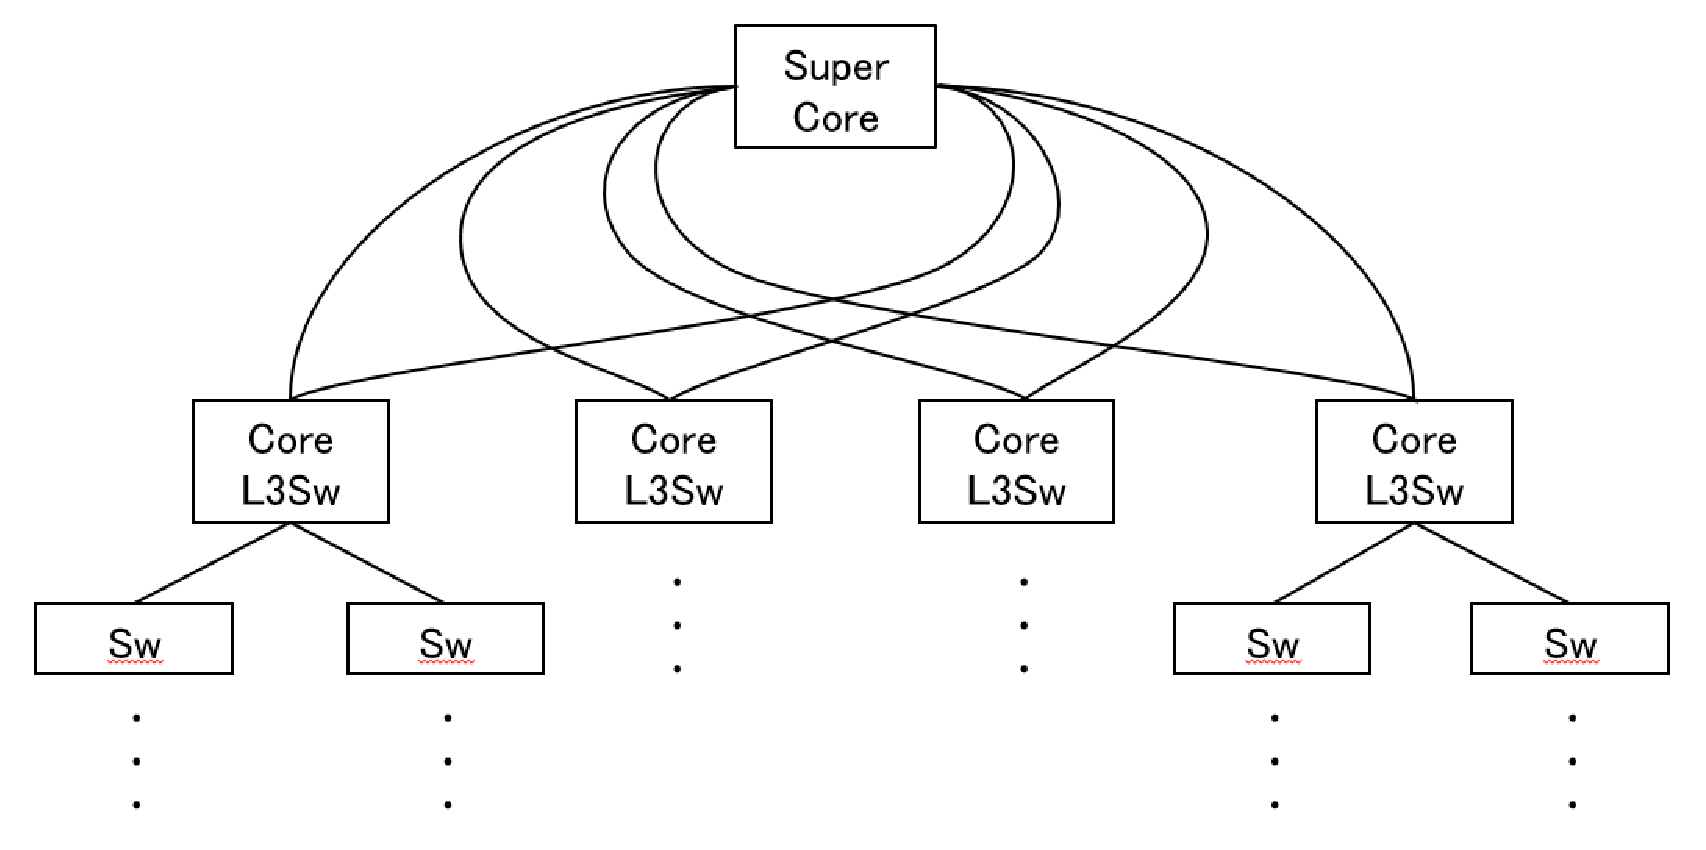
\includegraphics{./img/eps/3-0.eps}} 
\caption{現在のスーパーコアの設計}
\label{fig:3-0}
\end{center}
\end{figure}

一般的な通信は,任意の2つのホスト間のパケットの経路は往復ともに同じであるという対称な通信を行っているが,現在導入されているスーパーコアでは,パケットの入力ポートおよび出力ポートを明確に設定し,経路選択を行っているため,パケット通信の経路は対称でない.
このようなパケット通信は一般的なIPSでは正常に動作が保証されておらず,限られた一部のIPSでしか動作しない可能性がある.

\section{ネットワークモデル構築法}

本節では,上記の問題点があるスーパーコアを改善したネットワークモデルを構築する方法を説明する.

スイッチをOpenFlow対応スイッチへと変更してネットワークを構成し,2種類のOpenFlowコントローラによってスイッチを制御することで,以下の図 \ref{fig:3-1}のようなネットワークを構築する.
OpenFlowスイッチは,2種類のOpenFlowコントローラによって制御を行う.

\begin{figure}[tb]
\begin{center}
\scalebox{0.5}{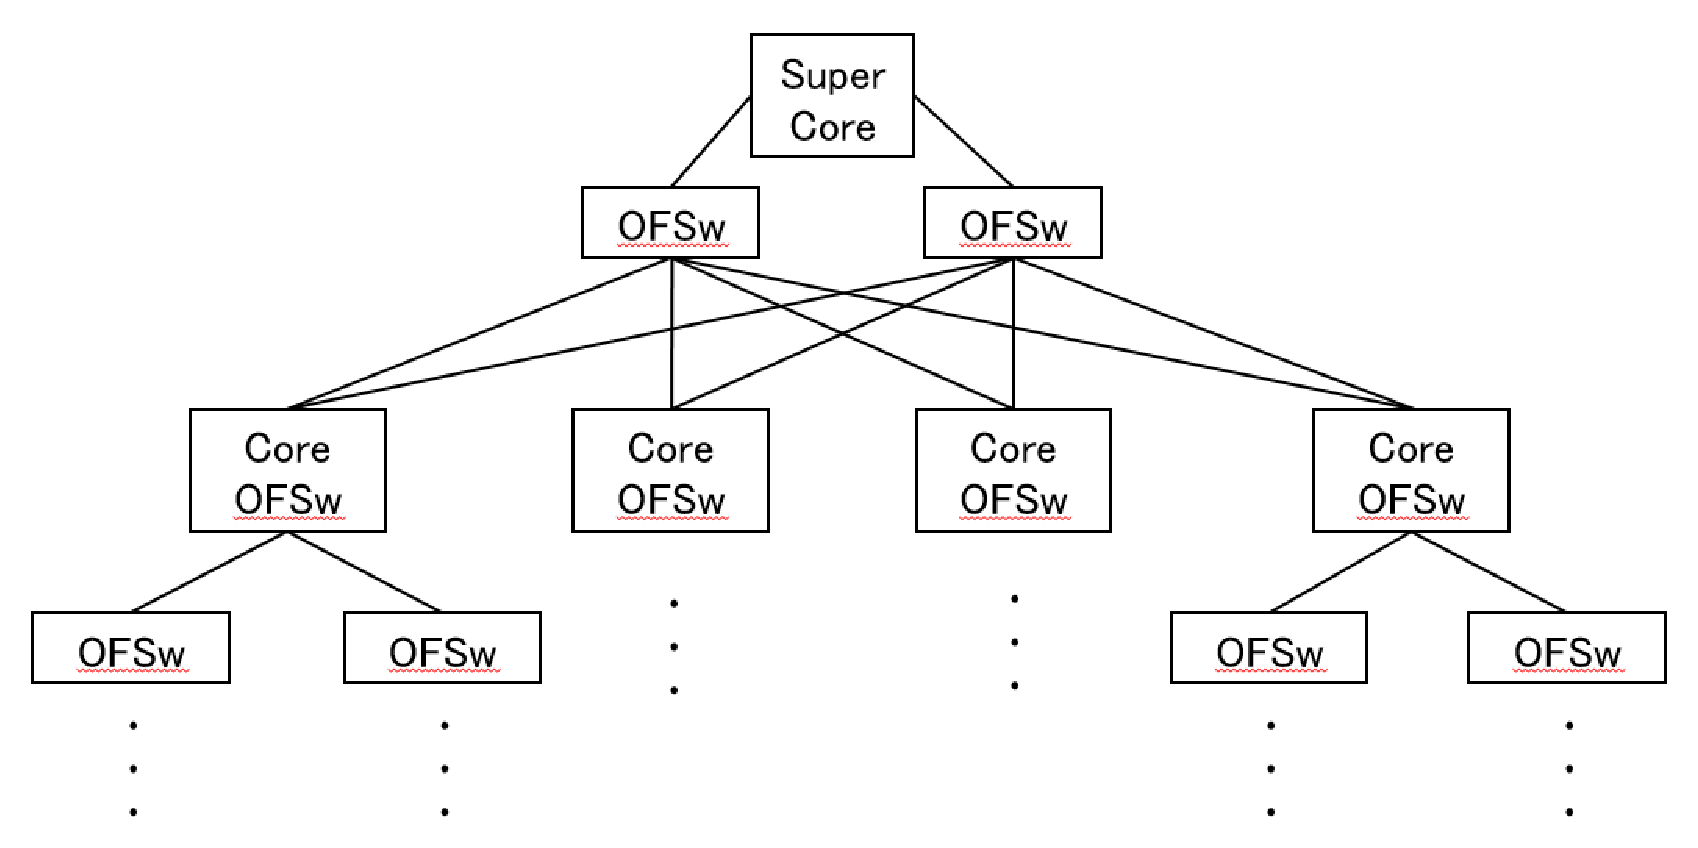
\includegraphics{./img/eps/3-1.eps}} 
\caption{提案するネットワークモデル}
\label{fig:3-1}
\end{center}
\end{figure}

次に,スイッチを制御する2種類のOpenFlowコントローラについて説明する.

\subsubsection{BasicController}

BasicControllerは,コアスイッチより下層に位置するスイッチ全て,および従来のスーパーコアとコアスイッチの間に新たに設置するスイッチを制御するOpenFlowコントローラである.
所属するOpenFlowスイッチは,物理ポートの1つを上層のネットワークと接続し,それ以外の物理ポートを下層のネットワークおよびホストと接続させることが必要.

下層のネットワークおよびホストから入力されたパケットを無条件で上層のネットワークへと出力し,上層のネットワークから入力されたパケットは,ルーティング規則に従い下層のネットワークおよびホストへと出力するという処理を行う.

\subsubsection{CoreSwitchController}

CoreSwitchControllerは,コアスイッチを制御するOpenFlowコントローラである.
コアスイッチは,物理ポート2つをスーパーコアとコアスイッチの間に新たに設置するスイッチ2つにそれぞれ接続し,それ以外の物理ポートを下層のネットワークと接続させる.

下層のネットワークから入力されたパケットは,上層のネットワークへ出力する際に,MACアドレスの比較を用いて出力する物理ポートを決定する.
パケットから送信元MACアドレスと宛先MACアドレスを取り出し,送信元MACアドレスの方が小さい場合は物理ポート0から,大きい場合は物理ポート1から出力するように処理を行う.
MACアドレスは各ネットワーク機器に対して,唯一かつ一意に割り振られているため,通信を行う任意のホスト2台間の通信経路は一意に決定され,対称性が保証される.

上層のネットワークから入力されたパケットは,ルーティング規則に従い出力ポートを決定する.
このとき,上層のネットワークに出力しないように設定する必要がある.

% 結果
%#####################################################################
\chapter{OpenFlowを用いたネットワークモデルの動作検証}
%#####################################################################

% 森定さんの内容
\begin{comment}
 本研究では,シミュレーションによってns-3上でEUNETを構築し,シミュレーションを行うことを目的としている.
シミュレーションは,実際のEUNETをモデル化して構築した上でパケットをキャプチャする事で性能を評価する事ができるようになる.

本章では,EUNETを再現するために作成したモジュールをどのように利用してトポロジを構築し,動作確認を行ったか解説する.\\

\section{各モジュールの動作確認}

本研究では3章で説明したようにns-3上でモジュールをC++で記述する事により作成しており,そのモジュールの組み合わせで意図するネットワークを構築していく.
そのため前提条件として,各モジュールが正常に動作する事が求められる.
そこで,作成したモジュールを用いて単純なネットワークを構成し,そのネットワークでのパケットの振る舞いを検証する事でモジュールが正常に動作しているかを確認した.\\
その際使用したテストコードを解説し,その結果を示す.実際に使用したテストコードは付録参照.

\subsection{EunetTestにおけるテストシナリオ}

動作確認を行うネットワーク機器は端末,L2スイッチ,L3スイッチの3つである.この機器を用いてネットワークを構成する.
端末はUDPで通信をおこなっており,パケットロスが生じた場合は再送を行わない.

\begin{figure}[tb]
\begin{center}
\scalebox{0.6}{\includegraphics{testsuit構成図.eps}} 
\caption{テストシナリオ構成}
\label{テストシナリオ構成}
\end{center}
\end{figure}

テストにおける構成は,図\ref{テストシナリオ構成}に記述している.
L3スイッチは3つ作成する.各L3スイッチはr1,r2,r3という名前を付け全てのL3スイッチは隣接して接続されている.
テストケースではr1,r3は以下に複数のL2スイッチ,端末を持つ.これを二つのエリアとみなし,ルーチングを行うことが可能か確認を行う.

L2スイッチは,両エリア下にスイッチを3つずつ接続を行う.エリア1におけるスイッチはs11,s12,s13,エリア2におけるL2スイッチはs21,s22,s23と名づける.この時L2スイッチは2階層の2分木であり,s11,s21は木の根部分となる.
そしてs11,s21はL3スイッチであるr1,r2にそれぞれ接続する.各L2スイッチには7つのポートがあり,L3スイッチおよびL2スイッチに接続していないポートには端末が接続されており.PacketSink,OnOffアプリケーションを持つ.\\

L3スイッチとL2スイッチの接続では回線速度が10Gbpsに,L2スイッチと端末,L2スイッチ同士の接続では回線速度を1Gbpsに設定している.
今回のテストシナリオでは,3つの動作確認を行う.
一つ目の動作確認はエリア1において,スイッチを3つ経由してパケットの送受信を行う端末の動作確認である.
s13下の端末であるt133がs12下の端末t125へパケットを送信する.そしてt133の送信パケット数とt125の受信パケット数を比較し,全てのパケットが受信できたのか確認を行う.


二つ目の動作確認は上述の端末に関する動作をエリア2において確認する.
送信を行うのはs22下のt225,受信はs23下のt233である.

三つ目の動作確認は上記二つの確認ができた場合に行われる.
L3スイッチを経由して接続されている端末間での送受信が行えるか確認を行う.
その際送信を行うのはエリア1のs12下にあるt125,受信を行うのはエリア2のs23下にあるt233である.
この動作確認ではr1,r3のルーチングテーブルが作成される前にパケット送信を行うとパケットロスが生じてしまうため,t233がパケットを受信しているかの確認を行う.

以上の3つの動作確認を行い,一つでも確認できなかった場合は,テストケースが中断されるようになっている.
テストケースを実行した結果,正常終了したので端末の動作,L2スイッチ,L3スイッチが動作していると判断した.


% 端末モジュールは各Terminalクラスを継承する事で構成され,EUNETにおける端末,すなわちエンドユーザが利用するPCを表現する.
% 3章で解説を行ったEunetTerminalクラスを用いて表現する.端末はOnOffNodeにて記述したランダムな時間パケットを送信,送信停止を行うOnOffアプリケーションと,PacketSinkNodeに記述した自身に向けて送信されたパケットを受信するPacketSinkアプリケーションを持つ.
% よって端末モジュールの動作確認を行う場合は,この2つのアプリケーションが正常に働いていることと,物理的,システム的に回線が接続されていることが確認できればよい.

% 今回の動作確認においては,2つの端末を直接接続し,パケットの送受信を行うことで動作確認を行い,ログを解析することで正常に動作していると確認できた.\\

% \subsection{L2スイッチモジュールの動作確認}

% L2スイッチモジュールは各Switchクラスを継承することで構成され,EUNETで使用されるL2スイッチを表現する.
% 3章で解説したように,L2スイッチの動作はルーチングテーブルに従い受け取ったパケットを宛先へ送信する事と,衝突が起こらないようデータを一時的にバッファすることである.
% L2スイッチの動作確認を行う際,端末が正常に動作していることが確認できていたので2つの端末をスイッチモジュールを介して接続し,端末モジュールのOnOffアプリケーションとPacketSinkアプリケーションを動作させ,パケットを送受信させることで動作確認を行った.

% 検証結果として,パケットの送受信ができていたので正常に動作していると判断した.

\subsection{L3スイッチモジュールの動作確認}

L3スイッチのルーチングアルゴリズムはDCEを利用しQuaggaデーモンを使用する.本研究では,L3スイッチはOSPFv2により経路情報を交換している.前述の動作確認のためのテストシナリオではPCAP形式でパケットをダンプしている.
このPCAPファイルを確認し,ルーチングアルゴリズムの振る舞いを検証する.

\begin{figure}[tb]
\begin{center}
\scalebox{0.6}{\includegraphics{ルータ動作確認Hello.eps}} 
\caption{ルータ動作確認(Helloメッセージ)}
\label{ルータ動作確認(Helloメッセージ)}
\end{center}
\end{figure}

図\ref{ルータ動作確認(Helloメッセージ)}はL3スイッチr1におけるPCAPファイルの一部である.
ここでr1は隣接ノードに対し,Helloメッセージにより自身の隣接ノードを伝えている.
この時点でr1に新たに隣接ノードr4が接続されていた場合,このHelloメッセージを受け取ったr4はr1の状態を把握できる.

\begin{figure}[tb]
\begin{center}
\scalebox{0.6}{\includegraphics{ルータ動作確認r1.eps}} 
\caption{ルータ動作確認(リンク状態更新)}
\label{ルータ動作確認(リンク状態更新)}
\end{center}
\end{figure}

図\ref{ルータ動作確認(リンク状態更新)}もr1におけるPCAPファイルの一部である.
ここでr1は自身の隣接ノードに対し,自身が接続されているネットワークについてのLS-Update(リンク状態更新)パケットをマルチキャストで送信し,
これに対するr3の応答を受け取っている.
これで,r1がOSPFに基づいて動作していることが確認でき,加えてr1のリンク状態をr3が把握していることも確認できる.

\begin{figure}[tb]
\begin{center}
\scalebox{0.6}{\includegraphics{L3スイッチ学習記録.eps}} 
\caption{L3スイッチ経路学習記録}
\label{L3スイッチ経路学習記録}
\end{center}
\end{figure}

図\ref{L3スイッチ経路学習記録}はテストケース実行時,L3スイッチにおけるルーチングテーブルの状況を示している.
この図では,シミュレーション開始から50秒経過時点では,各L3スイッチは経路が学習されておらず,自分が直結しているネットワークに対する経路情報しか学習していない.
60秒が経過すると,r1とr3の間では経路が学習され,2つのネットワークの間に経路ができる.
その結果,r1下にある端末とr3下にある端末が通信を行うことが可能となる事が確認できる.



これらの結果より,作成したL3スイッチを表現するテストモジュールが,OSPFv2を用いたルーチングを行い,動作している事が確認できた.

% \begin{figure}[tb]
% \begin{center}
% \scalebox{0.7}{\includegraphics{ルータ動作確認TCPパケット.eps}} 
% \caption{ルータ動作確認(TCPパケット)}
% \label{ルータ動作確認TCPパケット}
% \end{center}
% \end{figure}

% \begin{figure}[tb]
% \begin{center}
% \scalebox{0.7}{\includegraphics{ルータ動作確認UDPパケット.eps}} 
% \caption{ルータ動作確認(UDPパケット)}
% \label{ルータ動作確認UDPパケット}
% \end{center}
% \end{figure}

% L3スイッチモジュールは各Routerクラスを継承することで構成され,EUNETにおけるL3スイッチを表現する.
% L3スイッチモジュールの持つ機能としてEUNET独自のルーチングやVLANの実装等が課題であった.だが本研究で開発を行い,動作確認を行えたのはQuaggaデーモンを利用し,ルーチングテーブルに従って受け取ったパケットを宛先へと送信するSimpleRouterクラスまでである.
% SimpleRouterクラスの動作確認では,L2スイッチモジュールの動作確認と同じく2つの端末の間にSimpleRouterクラスにより作成されたモジュールを接続し,Quaggaデーモンを利用するモジュールを組み込み,そのルーチングにより宛先を把握し,データを送信するよう設定した.
% シミュレータ上で実際にパケットを流し,解析した結果,Quaggaデーモンが正しく動作していることが分かった.判断基準として,送信するパケットの種類をTCPパケットとUDPパケットを送信するシミュレーションをそれぞれ行った所,パケットの処理にかかる時間が違うこと,Helloメッセージに対して返信が行われており,パケットの送受信が成功している事が分かったため,SimpleRouterクラスが正常に動作していると判断した.図 \ref{ルータ動作確認TCPパケット} にTCPパケットの送受信ログを,図 \ref{ルータ動作確認UDPパケット} にUDPパケットの送受信ログを示す.衝突や信号誤りは存在しないが,パケットの処理工程の差により,応答時間に違いがみられる.\\


% \section{各クラスを用いたEUNETの再現・検証}

% \noindent\textgt{EunetSimulation}

% これまでに用意した各クラスを利用し,各キャンパスのエッジネットワークを記述したクラス.
% このクラスを用いて再現したネットワークは図 \ref{エッジネットワーク(重信キャンパス)} のように可視化される.

% \begin{figure}[tb]
% \begin{center}
% \scalebox{0.3}{\includegraphics{重信トポロジ.eps}} 
% \caption{エッジネットワーク(重信キャンパス)}
% \label{エッジネットワーク(重信キャンパス)}
% \end{center}
% \end{figure}

% 図 \ref{エッジネットワーク(重信キャンパス)} は末端ノードが端末(PC),親ノードがスイッチで構成されたテストケースである.
% 仕様書に記載されたようにC++でシナリオを記載していった.EUNETを再現し,可視化する事により全てネットワークの根が唯一となった.
% この事によりどのネットワークに所属している端末からでも,全ての端末と通信できる事が分かった.加えて,愛媛大学の全てのキャンパス,建物が同一のネットワークに接続されていると判明した.
% このテストケースで構成したトポロジを利用して端末にパケットを送信させた結果,ログの解析を行うことにより全ての端末がその他の端末との通信に成功していた.これにより設計したトポロジで,コネクションを確立しパケットの送受信が可能であると分かった.つまり,各モジュールの振る舞いをモデル化する事ができれば,EUNETの性能を評価する事ができる.
% 端末,スイッチを表現するモジュールに関しては動作も確認できている,これらを用いる事でns-3上にネットワークモデルを構築する事ができる.

% 本研究では,端末,スイッチの他にL3スイッチモジュールの開発を行った.SimpleRouterクラスの動作確認を行い,Quaggaデーモンを利用したルーチングを実装し,パケットの送受信を行うL3スイッチモジュールの作成まで完了した.
\end{comment}

% 自分の内容
 本研究は,ネットワークシミュレータ上であるns-3上でOpenFlowを用いたネットワークモデルを構築し、シミュレーションを行い、ネットワークモデルが正常に動作するかを検証することが目的である。
ns-3では、シミュレーションによるトラフィックの流れをキャプチャすることが可能であるため、これを用いて作成したネットワークモデルの動作の検証結果を本章で述べる。

\section{ネットワークモデルの動作検証}

動作検証を行う際に、以下の3つのケースを想定しテストコードを作成した。

\begin{itemize}
	\item 送信元と送信先のL3サブネットの所属が違うとき
	\item 送信元と送信先のL3サブネットの所属が同じとき
	\item 
\end{itemize}



% 結論
%#####################################################################
\chapter{まとめ・今後の課題}
%#####################################################################

 本章では,本研究の考察およびまとめを行い,本研究における今後の課題を述べる.

本研究は,スーパーコアに関して考案した新たなネットワークモデルの構築をネットワークシミュレータns-3上で行った.
当初の目標である,OpenFlowを用いてのスーパーコアを経由したパケット転送の制御は,検証結果を見てみると全て意図したアルゴリズムの通り問題なく実装されていると考えられる.
これにより,従来のスイッチのように複雑なテーブルを全て手動で制御することなく,大部分をコントローラに任せることができる.
更に,本研究で用いたネットワークモデルを用いることで,現在スーパーコアで使用されているIPSだけでなく,様々なIPSを用いて従来のような性能を期待できると考えられる.

本研究ではOpenFlowを用いたモデル構築の初期段階しか扱うことができなかったが,今後OpenFlowを用いた大規模なモデル構築をする際の一助となればよいと考える.
更に,ns-3を用いてネットワークモデルを構築するという内容に関する日本語論文およびテキスト,Webページが滅多に存在せず,更にOpenFlowを用いるという条件を加えるとその数は更に減少する.
本論文により,OpenFlowとns-3を用いたシミュレーションの一例が増えることに貢献できたと考える.
% 今後,技術が更に発展しOpenFlowが実用化に近づくことを切に願うばかりである.

最後に,本研究を行った上での今後の課題を以下に示す.

一つ目の課題として,構築したネットワークモデルと現EUNETとの詳細な仕様の乖離が挙げられる.
本研究では,通信されるパケットは全てスーパーコアを経由するという前提のもとで,ネットワークモデルを構築した.
しかし,現EUNETはVLANなどを用いてセグメントを分けるという処理を行っている.
ホスト間のセグメントが別ならば,通信されるパケットはスーパーコアを用いて検疫したのち,宛先のホストへと届けられるが,セグメントが同じならば,通常のスイッチおよびルータと同じように振る舞い,パケットを通信する.
つまり,OpenFlow技術を用いてEUNETを詳細に表現しシミュレーションするためには,以上のような仕様追加を行い,再度シミュレーションをする必要がある.

二つ目の課題は,OpenFlowスイッチ,コントローラおよびホストいずれも実機を用いた実験を行っていないということである.
2.1節で説明したように,ns-3ではTAPデバイスを用いることによって,シミュレーションモデルの一部を実機に繋ぐことができ,より現実的な実験を行うことができる.
実際にEUNETをOpenFlowを用いて構築しようとするとき,一般に市販されているOpenFlow対応スイッチおよびコントローラを用いることがほとんどであろう.
しかし,今回の実験では市販品を用いた実験ではなく,全てns-3および別添のOpenFlowモジュール群でサポートされているモジュールを用いてスイッチおよびコントローラを作成した.
つまり,本研究で提案した手法はそのまま引き継げる可能性があるが,作成したプログラムをそのまま適用できないことが考えられる.
更に本研究はOpenFlow 0.8.9というOpenFlowの中で一番古いバージョンを用いている.
OpenFlowの制約も,導入するときのバージョンによって異なる可能性があるため,今回の手法が現在のOpenFlow技術に対して有効的でない可能性があると考えられる.

% 謝辞
\acknowledgement

本研究を行うに当たり,情報基盤研究室の皆様には懇切なるご指導を頂き,大変お世話になりました.
特に,川原稔先生には,研究内容での議論の際に多くのご意見を賜り,本論文の内容の細部にいたるまでチェックして頂きました.
そして,佐々木隆志先生にはプログラムコードの作成の際に適切なご助言を頂き,大変お世話になりました.

研究スペースの提供などでお世話になりました愛媛大学総合情報メディアセンタの職員の皆様,研究室の皆様に感謝致します.

最後に,本研究に対して審査頂きました○○先生および○○先生に深くお礼申しあげます.

% 参考文献
 
\bibliographystyle{ipsjsort}
\bibliography{Bibliographies}
\nocite{*}


\end{document}